\section{Konzept}

\begin{figure}[hbtp]
\centering
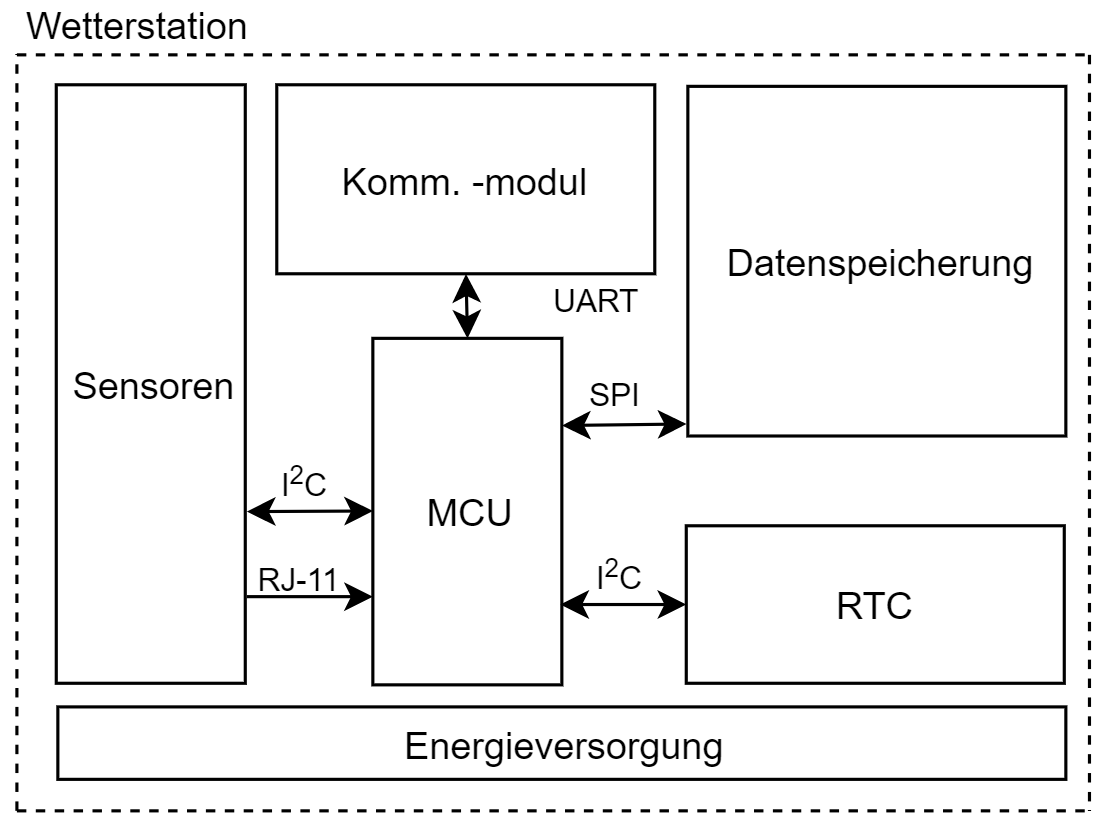
\includegraphics[width=0.9\textwidth]{graphics/Konzeptdiagramme/Grundkonzept.PNG}
\caption{Grundkonzept}
\label{fig:grundkonzept}
\end{figure}


Das gesamte Grundkonzept ist, wie in der Abbildung \ref{fig:grundkonzept} grafisch dargestellt, modular aufgebaut. Auf alle einzelnen Module wird folgend spezifischer eingegangen und genauer erklärt wie die partiellen Module funktionieren, sowie auch das gesamte System aufgebaut ist.\\

Als Zentralrecheneinheit wird eine \textit{Micro-Controller-Unit (MCU)} verwendet. Dieser ist dafür verantwortlich, dass die Daten richtig verarbeitet und an das dementsprechende Modul weitergeleitet werden. Die Messdaten werden in digitaler Form vom Modul \textit{Sensoren} über das I$^{2}$C-Interface an die \textit{MCU} übertragen. Dieser fügt mit dem \textit{Real-Time-Clock (RTC)} einen Timestamp hinzu, wobei anschließend die Daten in der \textit{Datenspeicherung} nichtflüchtig gespeichert werden. Über das \textit{Kommunikationsmodul} können dann die Daten von Nutznießern abgefragt werden.\\

Das Kommunikationsmodul beinhaltet momentan nur das USB-Interface für eine Kommunikation nach außen, wie auch zu Debbug-Zwecken des Programms. Auch die Energieversorgung wurde noch nicht implementiert und wurde folgend auch noch nicht genauer erläutert. Diese zwei Teile des Projektes werden in einem weiterführendem Projekt realisiert.\\

\newpage

\begin{figure}[hbtp]
\centering
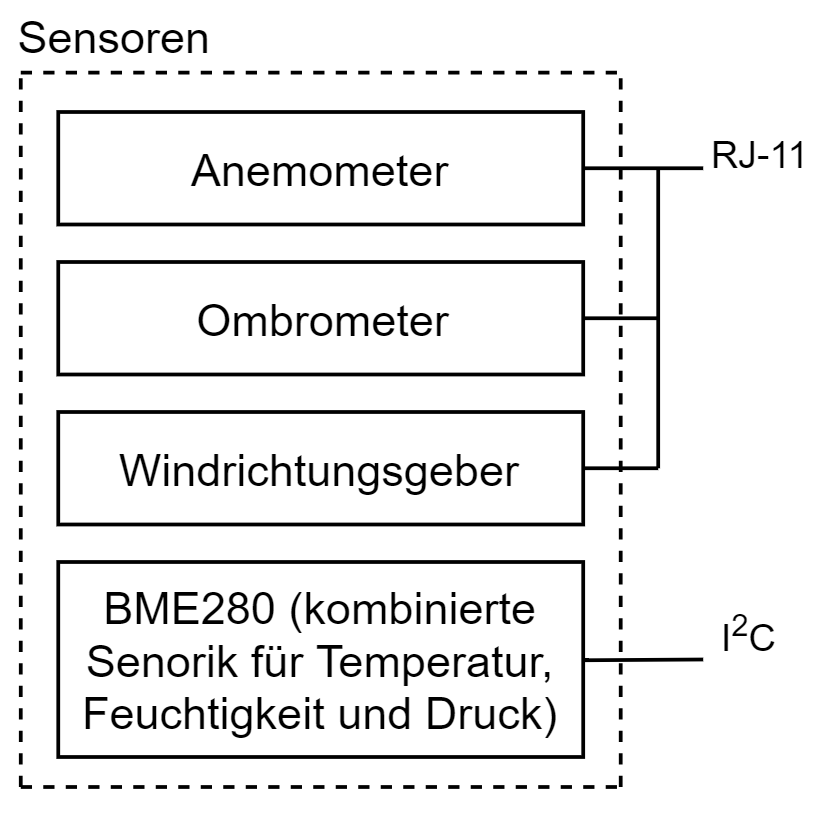
\includegraphics[width=0.6\textwidth]{graphics/Konzeptdiagramme/Sensoren.PNG}
\caption{Modul Sensoren mit den verwendeten Sensoren und Messfühlern}
\label{fig:Sensoren}
\end{figure}

Um eine bessere Übersicht über die verwendeten Sensoren zu geben, wie sie angeschlossen sind und wo sie sich in der gesamten Abstraktion des Konzeptes befinden dient Abb. \ref{fig:Sensoren}. Genauere Spezifikationen der Sensorik werden in den folgenden Kapiteln erläutert.

\newpage
\subsection{Prototyping}
\begin{figure}[hbtp]
\centering
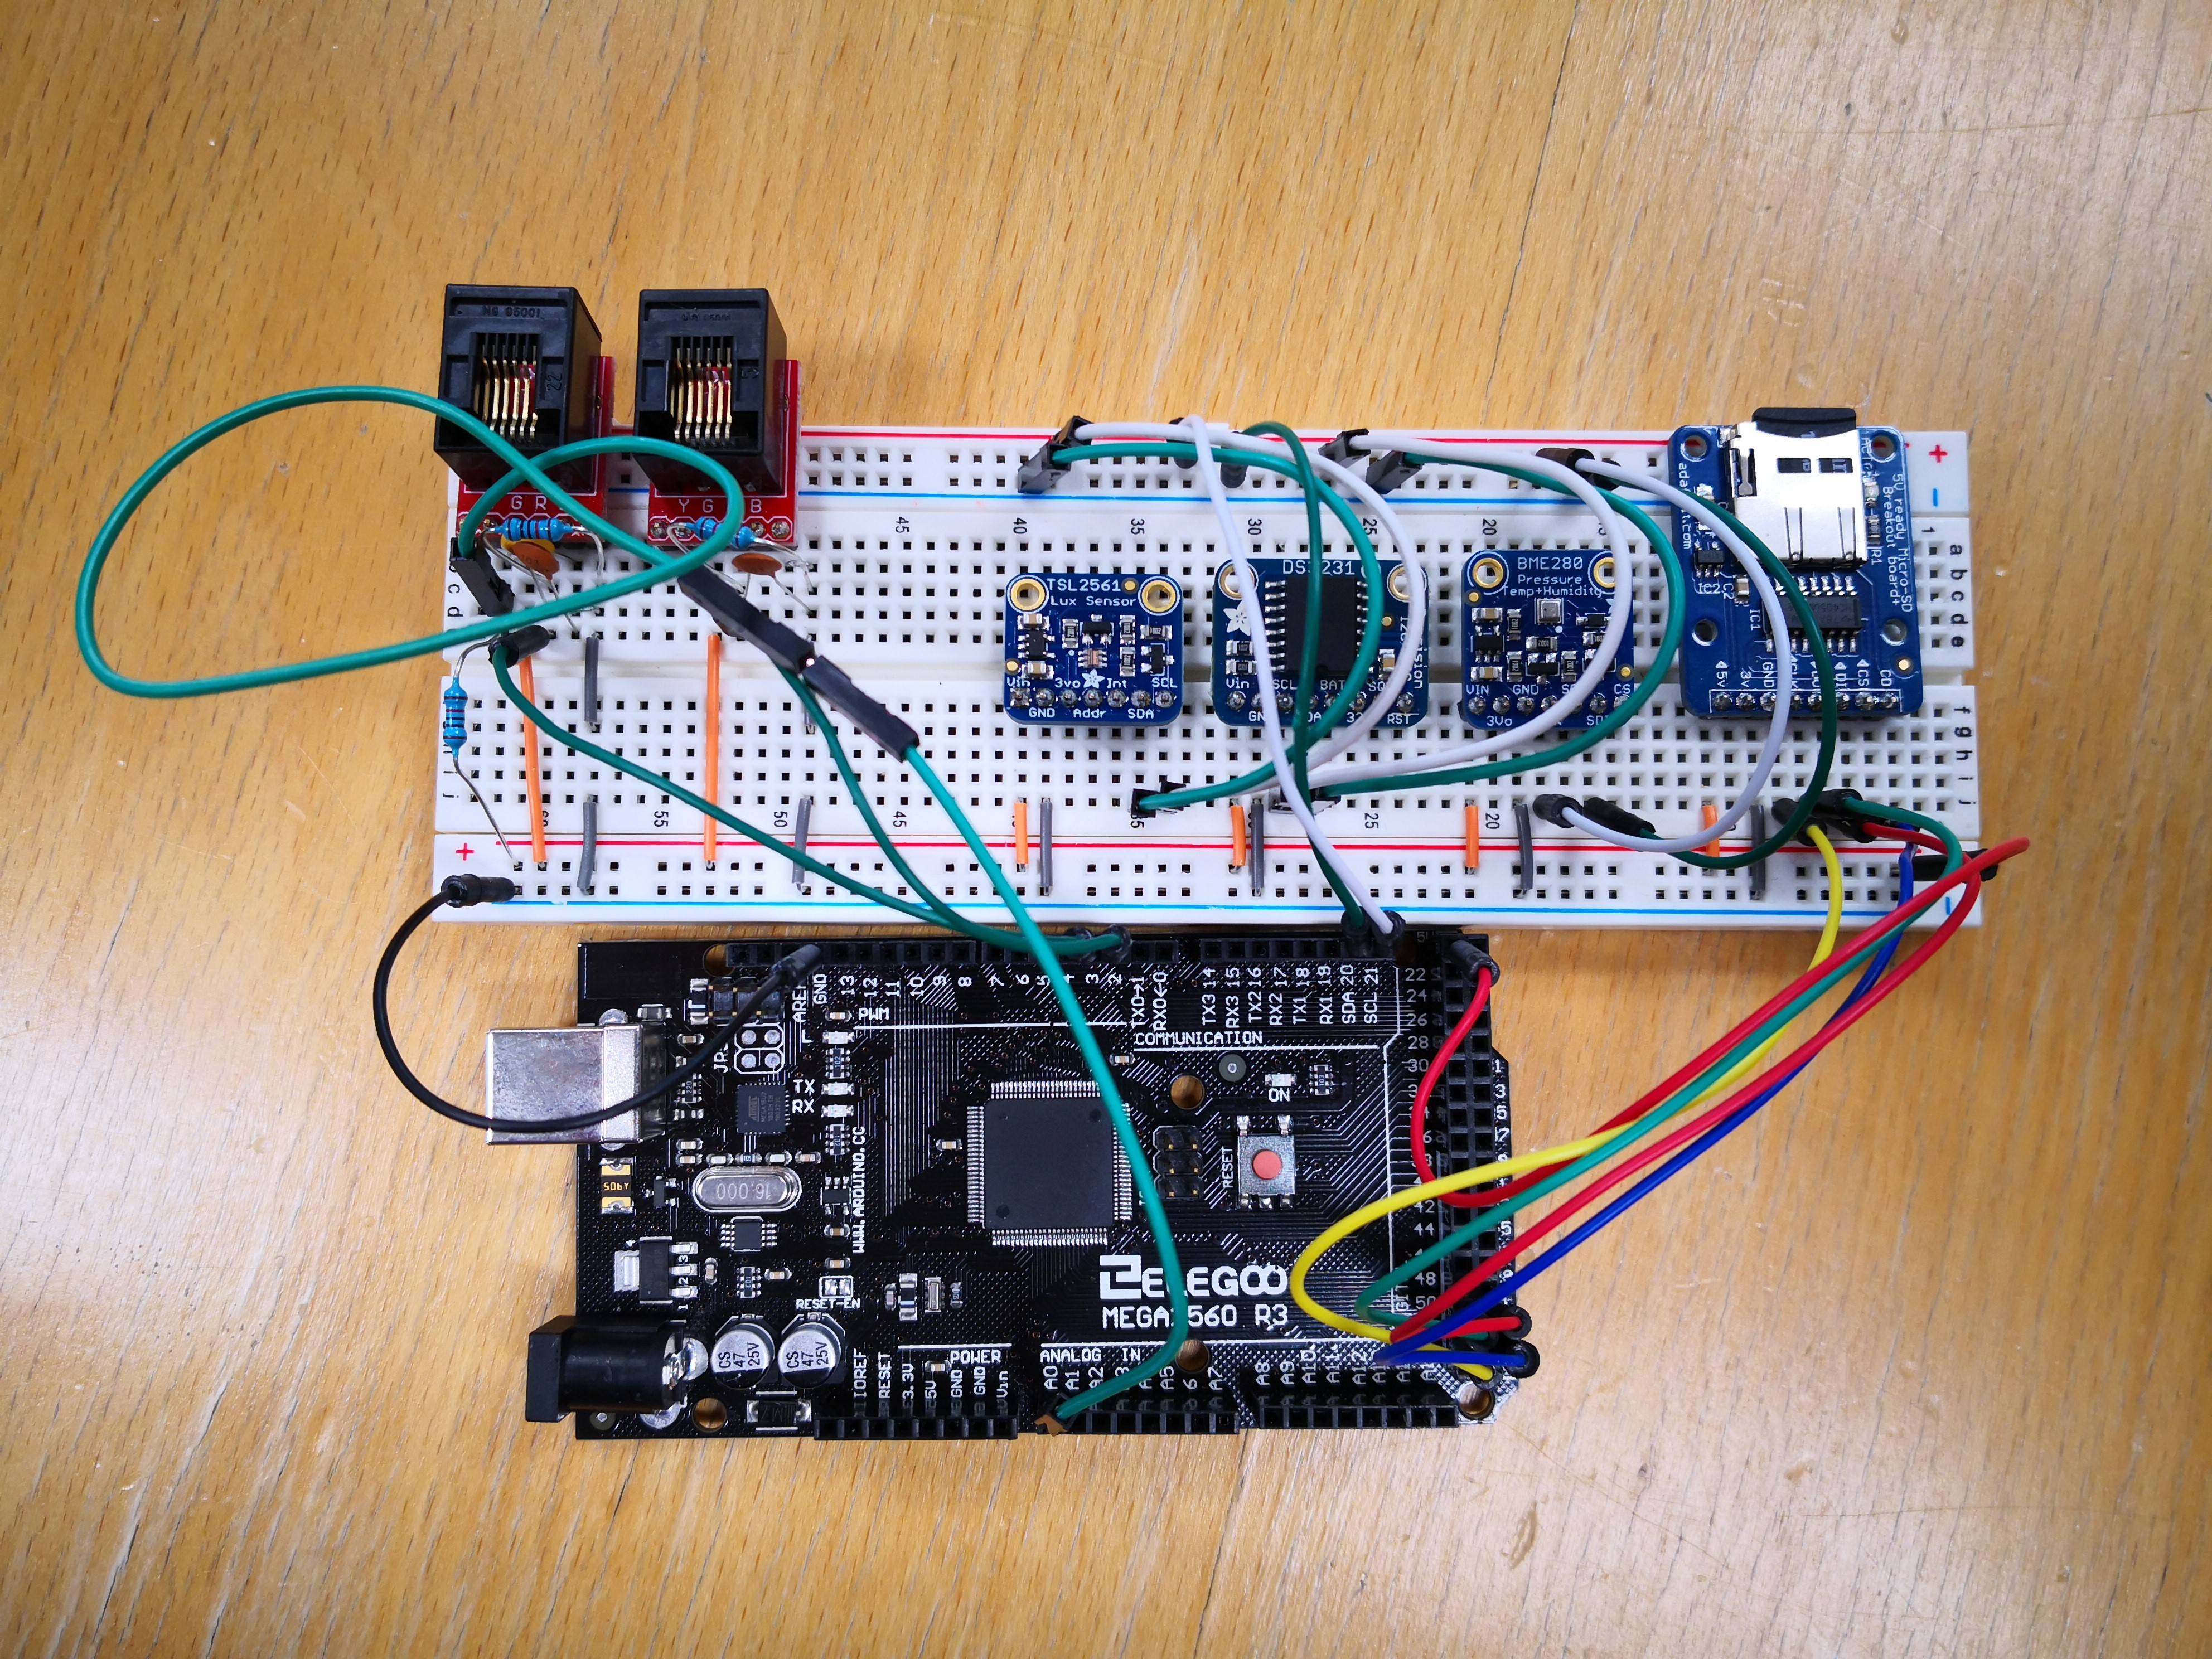
\includegraphics[width=0.9\textwidth]{graphics/prototyping/IMG_20190118_105725.jpg}
\caption{Prototyping mittels Breakoutboards}
\end{figure}
